% unspecified length
%Relevance:
% - voting behavior less well researched than elecotral voting behavior
% - referendums increasingly used
% - can citizens vote competently?
% - 

\documentclass[11pt,a4paper]{article}
\usepackage[utf8]{inputenc}
\usepackage{amsmath}
\usepackage{amsfonts}
\usepackage{amssymb}
\usepackage{graphicx}
\usepackage[round]{natbib}
\usepackage{url}
\usepackage{fullpage}
\usepackage{graphicx}

\author{Arndt Leininger \thanks{Hertie School of Governance, \texttt{a.leininger@phd.hertie-school.org}}}
\title{\Large{\textsc{Who votes against the government and why?}}\\ \large{\textsc{Voting Behavior in National Referendums in Switzerland}}} % Change title?
\date{}

\begin{document}

\maketitle

{\small \textit{Submitted for consideration for the Leuven-Montréal Winter School in Elections and Voting Behaviour 2015.}}


\begin{abstract}
    The proposed paper studies voting behavior in national referendums in Switzerland, more concretely what motivates voters to vote counter to the vote recommendations issued by the Swiss federal government. Voters vote in referendums more often and in more places than is commonly thought. Yet, voting in referendums has largely been a neglected topic in research on voting behavior which mostly focused on electoral behavior. The research that exists has focused on whether citizens are capable of casting an informed vote as levels of voter competence in referendums are thought to be even lower than in elections. This line of research has, counter to popular arguments against direct democracy, found that even uninformed citizens often are capable to vote in a way they would have voted had they been better informed on the issue at hand. Low-informed  voters are able to mimic informed voters' choices by relying on cues from governments, parties and interest groups.
    
    This paper is motivated by the observation that in Switzerland the effectiveness of such cues, concretely vote recommendations propagated by the Swiss government, has apparently decreased in effectiveness. Switzerland has since roughly the late 1970s experienced a secular upward trend in the number of referendums the government loses, both in absolute and relative terms (Fig. \ref{fig}). The initiatives on a ban on building minarets and the deportation of convicted non-Swiss citizens which were both opposed by the government but still approved by a majority of voters are only two prominent examples from recent times.
    
    I use the full cumulation of the VOX post-referendum surveys that cover all 246 national referendums held in Switzerland between 1981 and 2010 to analyze the individual and macro-level determinants of voting `against the government.' Given the state of the literature on referendum voting the paper is rather descriptive in nature. I focus on identifying the determinants of the above defined outcomes rather than precisely estimating a specific determinant.
    
    On the individual level I concentrate on citizens' political competence -- capturing how informed voters are about a referendum -- and political sophistication more generally -- how interested and informed citizens are about politics in general. In include the usual socio-economic covariates which in Switzerland include the politico-linguistic divide between the German and the French and to a lesser degree the Italian speaking Swiss population. 
    
    On the macro level I spotlight the type and topic of a referendum as well as the campaign waged by proponents and opponents in the lead-up to a referendum. While obligatory referendums are triggered by government action initiatives are a tool for interest groups to enact policies the legislature would not pass. Who triggers a referendum could have an effect on citizens' propensity to reject the policy favored by the government. On the topics considered in a referendum it has been suggested by many commentators that initiatives directed against minorities have proven particularly successful. Of particular relevance to parties and governments, lastly, is the question whether campaigns can encourage citizens to vote in the desired way.
    
    In the paper to be submitted to the winter school I will have developed these thoughts further and provide first results. I will also outline two potential extensions to the paper. Firstly, I articulate thoughts on how I could, among the voters `defying' the government, distinguish what I would call `reasoned' from `populist' deviators.  
    
    Secondly, I discuss how my initial results could contribute to explain the macro-level trend in rising numbers of government defeats. This trend could be rooted in both macro and individual level factors. For instance, if voters are more likely to vote against the government's recommendation if the referendum was triggered by an initiative there recent rise in initiatives (Fig. \ref{fig}) use could explain part of the rise in `defeats.' On the individual level, a decline in party identification in the voting population could explain why voters increasingly disregard their government's vote advice.

    
\end{abstract}

\small\textbf{Keywords: Referendums, Voting, Switzerland, Multi-level modelling}

\begin{figure}[htb]
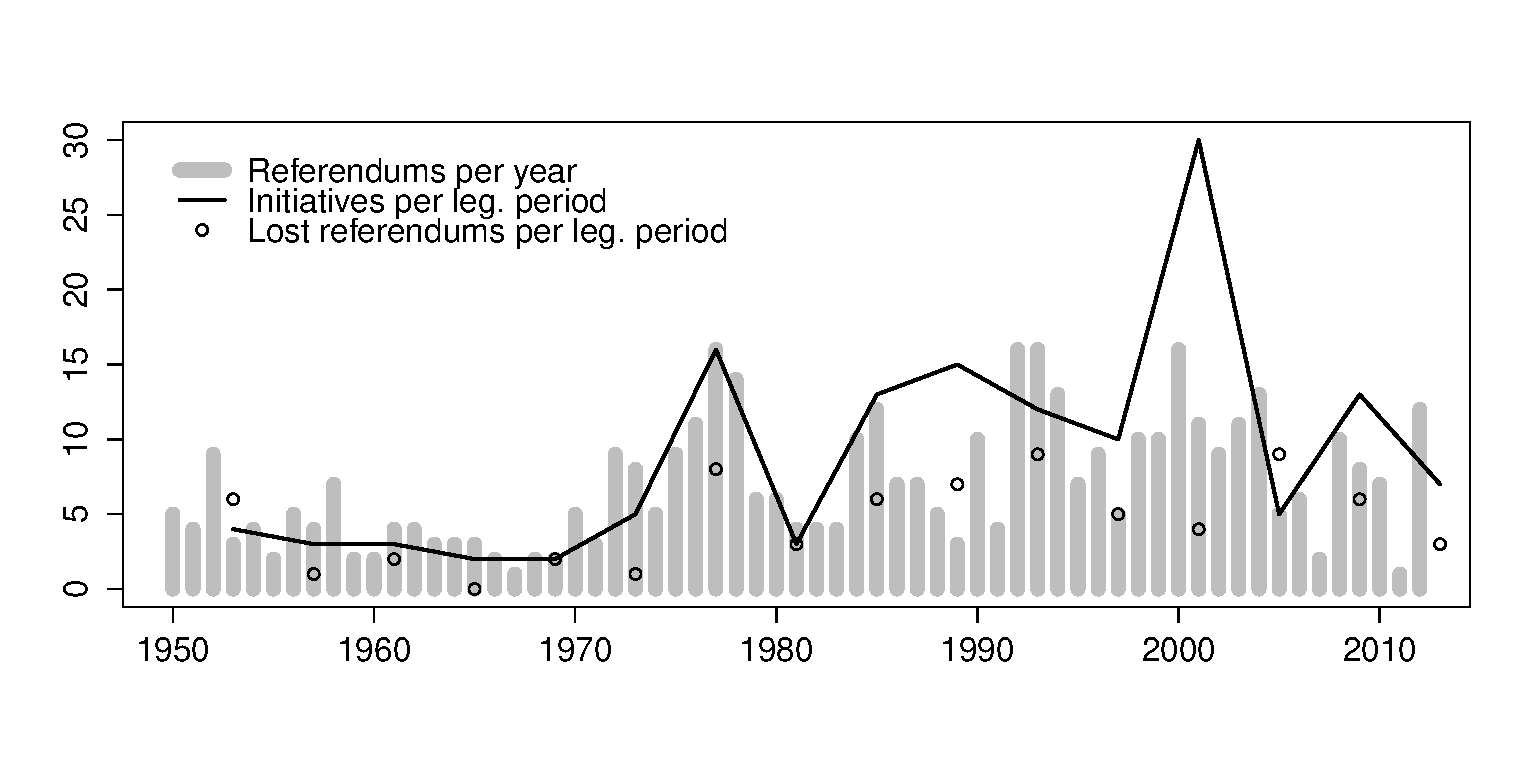
\includegraphics[width=\textwidth]{../../figures/figure.pdf}    
\caption{Number of national referendums, initiatives and referendums lost by the government in Switzerland (1950-2013). Counts per legislative period plotted at midpoint of legislative period.}\label{fig}
\end{figure}


\end{document}
